\documentclass[tikz,border=3pt]{standalone}
\usetikzlibrary{arrows.meta,decorations.markings}
\begin{document}
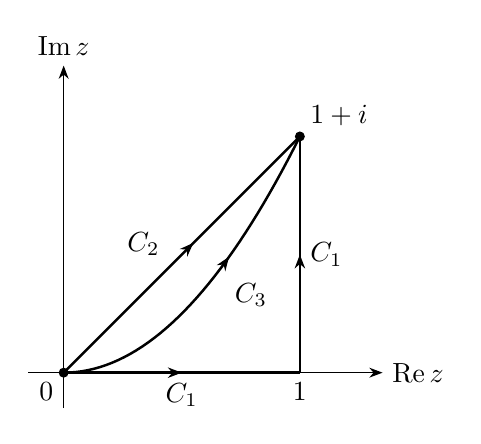
\begin{tikzpicture}[scale=3,>=Stealth,line width=0.9pt,
  mid/.style={postaction={decorate},decoration={markings,mark=at position #1 with {\arrow{Stealth[length=5pt]}}}}]
  \draw[line width=0.4pt,->] (-0.15,0) -- (1.35,0) node[right] {$\mathrm{Re}\,z$};
  \draw[line width=0.4pt,->] (0,-0.15) -- (0,1.3) node[above] {$\mathrm{Im}\,z$};
  \draw[mid=0.5] (0,0) -- (1,0);
  \draw[mid=0.5] (1,0) -- (1,1);
  \draw[mid=0.55] (0,0) -- (1,1);
  \draw[mid=0.6,domain=0:1,samples=40] plot (\x,{\x*\x});
  \fill (0,0) circle (0.6pt) node[below left] {$0$};
  \fill (1,1) circle (0.6pt) node[above right] {$1+i$};
  \node[below] at (1,0) {$1$};
  \node[below] at (0.5,0) {$C_1$};
  \node[right] at (1,0.5) {$C_1$};
  \node[above left] at (0.45,0.45) {$C_2$};
  \node[below right] at (0.68,0.42) {$C_3$};
\end{tikzpicture}
\end{document}
